\documentclass[letterpaper]{article}
\usepackage{iftex}
\ifPDFTeX
  % Submission path: use the unmodified official AAAI style with PDFLaTeX.
  \makeatletter
  \def\input@path{{../../../EGO_paper/EGO_AAAI27/}}
  \makeatother
  \usepackage[submission]{aaai2027}
\else
  % Portable preview path for Tectonic/XeTeX in environments without PDFLaTeX.
  % It mirrors the AAAI page and column geometry but is not a submission build.
  \usepackage[margin=0.75in,columnsep=0.375in]{geometry}
  \usepackage{authblk}
  \setlength{\affilsep}{0pt}
  \twocolumn
\fi
\usepackage[hyphens]{url}
\usepackage{graphicx}
\urlstyle{rm}
\def\UrlFont{\rm}
\usepackage{natbib}
\usepackage{caption}
\frenchspacing

\usepackage{booktabs}
\usepackage{amsmath}
\usepackage{amssymb}
\usepackage{xcolor}
\usepackage{tikz}

% DRAFT COLOR CONTRACT:
%   blue = measured value; red = preregistered claim rejected by the final result.
% Before submission, resolve the red claim in prose and redefine both macros
% as identity functions.
\definecolor{measuredblue}{RGB}{0,73,160}
\definecolor{pendingred}{RGB}{190,35,35}
\newcommand{\obs}[1]{\textcolor{measuredblue}{#1}}
\newcommand{\rejected}[1]{\textcolor{pendingred}{#1}}
\newcommand{\pp}{\,\mathrm{pp}}
\newcommand{\method}{\textsc{EGO}}
\newcommand{\cmark}{\checkmark}

\ifPDFTeX
  \pdfinfo{/TemplateVersion (2027.1)}
\fi
\setcounter{secnumdepth}{0}
\title{Results Draft: Embodied Reasoning as Grounded Selection}
\author{Anonymous Submission}
\ifPDFTeX
  \affiliations{Anonymous Affiliation}
\else
  \affil{Anonymous Affiliation}
\fi

\begin{document}
\setlength{\emergencystretch}{1em}
\maketitle

\section{Results}
\subsection{Embodied Reasoning}
\label{sec:er-capability}

\paragraph{Evaluation protocol and evidential order.}
We evaluate at anticipation points from the Ego4D GoalStep held-out split.
The frozen world model receives the observation and completed-action history,
then proposes a shuffled Top-$K$ action boundary; its scores and ranks are
hidden from the policy.  Unless noted otherwise, all comparisons use the same
first-person evaluation cohort and the common covered set
($a_t^{\mathrm{GT}}\!\in D_t$; \obs{$n{=}1{,}000$}).
We organize the evidence from outcome to mechanism: first the controlled
selection comparison, then capability decomposition, and finally paired
interventions on history and task belief.  This order separates an improvement
in \emph{what is selected} from a superficial change in \emph{how the trace is
written}.

\subsubsection{Candidate Alignment, Not Answer-Only Supervision, Improves Selection}
\label{sec:er-selection}

The primary comparison controls backbone, examples, training budget, and
evaluation prompts; the only change is whether training exposes the
world-model candidate set.  Candidate alignment
($\theta_{\mathrm{CE}}$) reaches \obs{$28.8\%$} selection accuracy, compared
with \obs{$21.9\%$} for answer-only supervision (GT-only).  On the official
non-malformed paired set (\obs{$n{=}948$}, 85 video clusters) their difference
is \obs{$+7.70\pp$}, with a video-cluster bootstrap
\obs{$95\%$ CI $[+3.73,+11.93]$}.  In contrast, GT-only differs from the
unaligned policy by only \obs{$+0.9\pp$}
(\obs{$95\%$ CI $[-2.0,+3.7]$}).  Candidate alignment also exceeds the frozen
world-model Top-\obs{$1$} policy (\obs{$28.8\%$} vs.\ \obs{$24.2\%$};
\obs{$+4.6\pp$} strictly); the official paired gate gives \obs{$+6.06\pp$}
(\obs{$95\%$ CI $[+0.87,+11.22]$}; \obs{$n{=}957$}, 86 clusters).  Thus, the
gain cannot be explained by additional exposure to the correct answer or by
copying the world-model ranking: it requires learning to discriminate among
visually plausible alternatives.  Figure~\ref{fig:capability}b traces SelAcc
along the branching training path: candidate alignment is the step that
carries the policy across the world-model reference.

\begin{figure*}[t]
\centering
\resizebox{0.96\textwidth}{!}{%
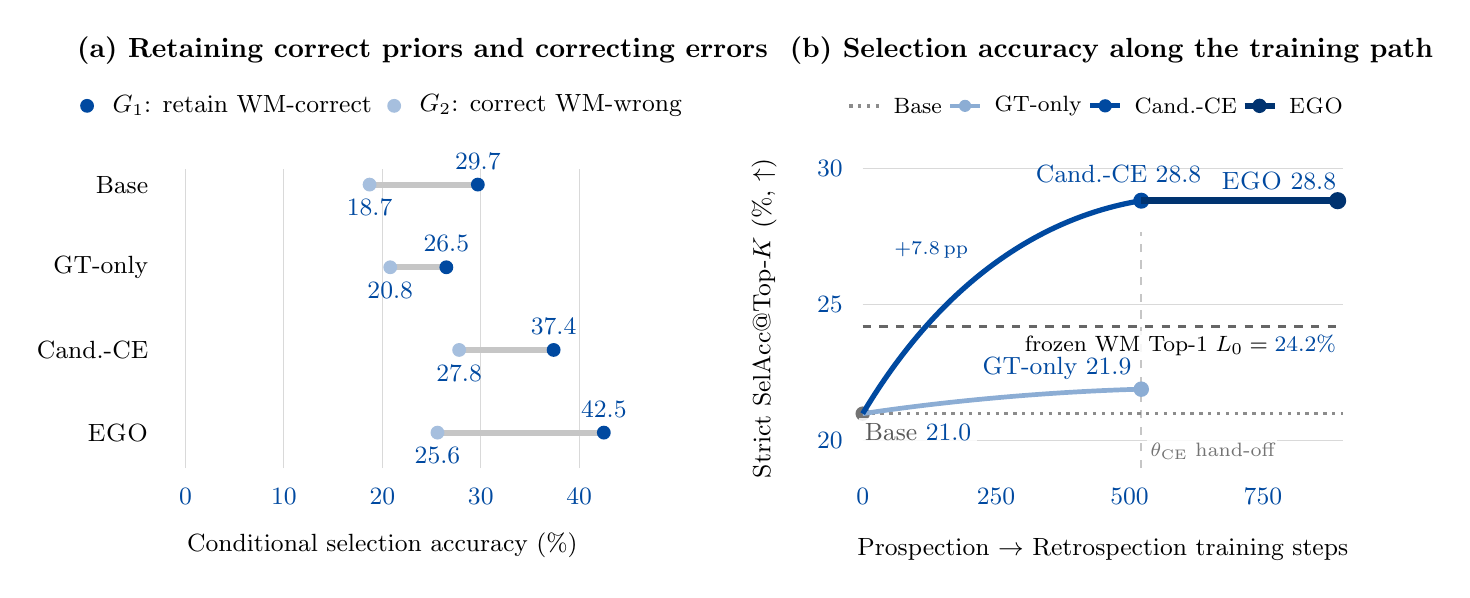
\begin{tikzpicture}[x=1cm,y=1cm,font=\small]
  % Panel (a): a dedicated title row, legend row, and plotting region.
  \node[anchor=west,font=\bfseries] at (0,6.15)
    {(a) Retaining correct priors and correcting errors};
  \fill[measuredblue] (0.25,5.45) circle (2.5pt);
  \node[anchor=west] at (0.45,5.45) {$G_1$: retain WM-correct};
  \fill[measuredblue!35] (4.15,5.45) circle (2.5pt);
  \node[anchor=west] at (4.35,5.45) {$G_2$: correct WM-wrong};

  \foreach \x/\lab in {1.5/0,2.75/10,4.0/20,5.25/30,6.5/40}{
    \draw[gray!30] (\x,0.85) -- (\x,4.65);
    \node[anchor=north,text=measuredblue] at (\x,0.72) {\lab};
  }
  \node[anchor=north] at (4.0,0.15) {Conditional selection accuracy (\%)};
  \node[anchor=east] at (1.15,4.45) {Base};
  \node[anchor=east] at (1.15,3.40) {GT-only};
  \node[anchor=east] at (1.15,2.35) {Cand.-CE};
  \node[anchor=east] at (1.15,1.30) {\method{}};

  \foreach \y/\gOne/\gTwo in {
    4.45/5.2125/3.8375,
    3.40/4.8125/4.10,
    2.35/6.175/4.975,
    1.30/6.8125/4.70}{
    \draw[line width=2.2pt,gray!45] (\gTwo,\y)--(\gOne,\y);
    \fill[measuredblue!35] (\gTwo,\y) circle (2.5pt);
    \fill[measuredblue] (\gOne,\y) circle (2.5pt);
  }
  \node[above=2pt,text=measuredblue] at (5.2125,4.45) {\obs{$29.7$}};
  \node[below=2pt,text=measuredblue] at (3.8375,4.45) {\obs{$18.7$}};
  \node[above=2pt,text=measuredblue] at (4.8125,3.40) {\obs{$26.5$}};
  \node[below=2pt,text=measuredblue] at (4.10,3.40) {\obs{$20.8$}};
  \node[above=2pt,text=measuredblue] at (6.175,2.35) {\obs{$37.4$}};
  \node[below=2pt,text=measuredblue] at (4.975,2.35) {\obs{$27.8$}};
  \node[above=2pt,text=measuredblue] at (6.8125,1.30) {\obs{$42.5$}};
  \node[below=2pt,text=measuredblue] at (4.70,1.30) {\obs{$25.6$}};

  % Panel (b): SelAcc against training steps, in panel (a)'s blue family.
  % x maps 0--900 optimizer steps onto 1.05--7.15cm: x(s) = 1.05 + s*0.0067778
  %   (s=522 -> 4.588 = theta_CE hand-off; s=890 -> 7.082 = end of Retrospection).
  % y maps 19--30% onto 0.85--4.65cm: y(v) = 0.85 + (v-19)*0.345455.
  % Markers are evaluated states only; curves interpolate between them.
  \begin{scope}[xshift=9.05cm]
    \node[anchor=west,font=\bfseries] at (0,6.15)
      {(b) Selection accuracy along the training path};

    \begin{scope}[font=\footnotesize]
      \draw[black!45,dotted,line width=1.2pt] (0.88,5.45) -- (1.26,5.45);
      \node[anchor=west] at (1.32,5.45) {Base};
      \draw[measuredblue!45,line width=1.5pt] (2.16,5.45) -- (2.54,5.45);
      \fill[measuredblue!45] (2.35,5.45) circle (2.2pt);
      \node[anchor=west] at (2.60,5.45) {GT-only};
      \draw[measuredblue,line width=1.7pt] (3.94,5.45) -- (4.32,5.45);
      \fill[measuredblue] (4.13,5.45) circle (2.4pt);
      \node[anchor=west] at (4.38,5.45) {Cand.-CE};
      \draw[measuredblue!70!black,line width=2.3pt] (5.90,5.45) -- (6.28,5.45);
      \fill[measuredblue!70!black] (6.09,5.45) circle (2.6pt);
      \node[anchor=west] at (6.34,5.45) {\method{}};
    \end{scope}

    \foreach \y/\lab in {1.1955/20,2.9227/25,4.65/30}{
      \draw[gray!30] (1.05,\y) -- (7.15,\y);
      \node[anchor=east,text=measuredblue] at (0.92,\y) {\lab};
    }
    \node[rotate=90,anchor=south] at (0.08,2.75)
      {Strict SelAcc@Top-$K$ (\%, $\uparrow$)};
    \foreach \x/\lab in {1.05/0,2.744/250,4.439/500,6.133/750}{
      \node[anchor=north,text=measuredblue] at (\x,0.72) {\lab};
    }
    \node[anchor=north] at (4.10,0.08)
      {Prospection $\rightarrow$ Retrospection training steps};

    % The two Retrospection runs branch from the same theta_CE adapter.
    \draw[gray!45,dashed,line width=0.7pt] (4.588,0.85) -- (4.588,3.85);
    \node[anchor=south west,font=\scriptsize,text=black!55,fill=white,
          fill opacity=0.85,text opacity=1,inner sep=1pt]
      at (4.66,0.92) {$\theta_{\mathrm{CE}}$ hand-off};

    % Frozen world-model Top-1 horizon.
    \draw[black!60,dashed,line width=1.0pt] (1.05,2.6464) -- (7.15,2.6464);
    \node[anchor=north east,font=\footnotesize,fill=white,fill opacity=0.86,
          text opacity=1,inner sep=1.5pt] at (7.12,2.60)
      {frozen WM Top-1 $L_0=\obs{24.2\%}$};

    % Base: frozen backbone, constant by construction, shared origin.
    \draw[black!45,dotted,line width=1.2pt] (1.05,1.5409) -- (7.15,1.5409);
    \fill[black!55] (1.05,1.5409) circle (2.6pt);
    \node[anchor=north west,inner sep=2pt,text=black!65,fill=white,
          fill opacity=0.85,text opacity=1] at (1.00,1.49) {Base \obs{$21.0$}};

    % GT-only: answer-only selection CE over the Prospection phase.
    \draw[measuredblue!45,line width=1.7pt]
      (1.05,1.5409) .. controls (2.10,1.70) and (3.40,1.82) .. (4.588,1.8518);
    \fill[measuredblue!45] (4.588,1.8518) circle (2.8pt);
    \node[anchor=south east,inner sep=2pt,text=measuredblue]
      at (4.54,1.90) {GT-only \obs{$21.9$}};

    % Cand.-CE: candidate-aligned selection CE over the same phase.
    \draw[measuredblue,line width=1.9pt]
      (1.05,1.5409) .. controls (2.10,3.30) and (3.40,4.05) .. (4.588,4.2455);
    \fill[measuredblue] (4.588,4.2455) circle (2.9pt);
    \node[above=3pt,text=measuredblue] at (4.30,4.2455) {Cand.-CE \obs{$28.8$}};
    \node[font=\scriptsize,fill=white,inner sep=1pt,text=measuredblue]
      at (1.92,3.62) {\obs{$+7.8\pp$}};

    % EGO: Retrospection with replay and grounding oversampling.
    \draw[measuredblue!70!black,line width=2.5pt]
      (4.588,4.2455) -- (7.082,4.2455);
    \fill[measuredblue!70!black] (7.082,4.2455) circle (3.1pt);
    \node[anchor=south east,inner sep=2pt,text=measuredblue]
      at (7.14,4.31) {\method{} \obs{$28.8$}};
  \end{scope}
\end{tikzpicture}
}
\caption{\textbf{Candidate alignment teaches grounded selection rather than
an answer prior.}  (a) $G_1$ evaluates retention where the world-model
Top-\obs{$1$} is correct, whereas $G_2$ evaluates correction where it is
wrong.  Candidate alignment improves both; GT-only erodes $G_1$ despite
seeing the correct answers, while the final \method{} model reaches
\obs{$42.5\%$} retention.  (b) Strict SelAcc@Top-$K$ against training steps
along the branching training path.  All arms share the same frozen origin
(\obs{$21.0\%$}).  Over the Prospection phase (\obs{$522$} selection-CE
steps) candidate alignment reaches \obs{$28.8\%$} whereas the answer-only
control reaches only \obs{$21.9\%$}.  \method{} then branches from the
$\theta_{\mathrm{CE}}$ adapter and trains a further \obs{$368$} steps of
Retrospection-with-Replay ($\rho{=}0.15$), holding \obs{$28.8\%$}.  Base is
frozen and is therefore constant by construction.  Lines are guides to the
eye.  Candidate alignment is the step that carries the policy across the
dashed frozen-WM Top-1 reference $L_0=\obs{24.2\%}$
(\obs{$+7.8\pp$}), and Retrospection preserves that position.}
\label{fig:capability}
\end{figure*}

\subsubsection{Where the Gain Appears: Five Capability Axes}
\label{sec:er-axes}

Aggregate accuracy alone does not reveal whether the policy preserves a
correct predictive prior or repairs an incorrect one.  We therefore split
selection into $G_1$ retention (world-model Top-\obs{$1$} correct) and $G_2$
correction (world-model Top-\obs{$1$} wrong).  As shown in
Figure~\ref{fig:capability}a and Table~\ref{tab:capability}, candidate alignment
raises $G_1$ from \obs{$29.7\%$} to \obs{$37.4\%$} and $G_2$ from
\obs{$18.7\%$} to \obs{$27.8\%$}.  GT-only instead lowers $G_1$ to
\obs{$26.5\%$}, even though it slightly raises $G_2$ to \obs{$20.8\%$}.
The final \method{} model further raises $G_1$ to \obs{$42.5\%$},
while $G_2$ settles at \obs{$25.6\%$}.
Providing a predictive boundary at inference is therefore insufficient:
the policy must be trained to recognize when that boundary's leading
hypothesis should be kept and when it should be overridden.

\begin{table*}[t]
\centering
\small
\setlength{\tabcolsep}{5pt}
\begin{tabular}{p{0.255\textwidth}ccccc}
\toprule
Capability metric & Base & GT-only & Cand.-CE & \method{} & What it tests \\
\midrule
SelAcc@Top-$K$ (\%, $\uparrow$)
  & \obs{$21.0$} & \obs{$21.9$} & \textbf{\obs{$28.8$}}
  & \textbf{\obs{$28.8$}} & overall grounded selection \\
$G_1$: retain WM-correct (\%, $\uparrow$)
  & \obs{$29.7$} & \obs{$26.5$} & \obs{$37.4$}
  & \textbf{\obs{$42.5$}} & preserve a valid predictive prior \\
$G_2$: correct WM-wrong (\%, $\uparrow$)
  & \obs{$18.7$} & \obs{$20.8$} & \textbf{\obs{$27.8$}}
  & \obs{$25.6$} & reselect beyond WM Top-\obs{$1$} \\
Continuation recall (\%, $\uparrow$)
  & \obs{$28.4$} & \obs{$32.9$} & \obs{$43.5$}
  & \textbf{\obs{$48.4$}} & recover trajectory-consistent action \\
Continuation precision (\%)
  & \obs{$72.7$} & \obs{$71.3$} & \obs{$71.1$}
  & \obs{$68.2$} & signal reliability (control) \\
Evidence utility (\(\Delta\) accuracy, pp, $\uparrow$)
  & \obs{$+13.5$} & \obs{$+3.2$} & \obs{$+12.3$}
  & \textbf{\obs{$+18.3$}} & evidence-to-decision coupling \\
Evidence mention rate (\%)
  & \obs{$22.4$} & \obs{$37.8$} & \obs{$32.4$}
  & \obs{$17.5$} & surface frequency (control) \\
Belief--action echo (\%, $\downarrow$)
  & \obs{$0.0$} & \obs{$28.8$} & \obs{$2.1$}
  & \textbf{\obs{$0.0$}} & belief content beyond action copy \\
\bottomrule
\end{tabular}
\caption{\textbf{Capability profile on the common covered set}
(\obs{$n{=}1{,}000$}).  Columns correspond to the unaligned policy, the
answer-only control, the candidate-aligned policy, and the final \method{}
model, respectively.  Continuations form
\obs{$31.0\%$} of the set
(\obs{$310/1{,}000$}); their stable precision shows that the main limitation
is recovery, not noisier continuation guesses.  Evidence utility is the
SelAcc difference between traces that do and do not explicitly invoke a
prior-action pattern; it is observational, not a causal effect.  Because the
world-model pool covers \obs{$43.4\%$} of held-out anticipation points, the
full-set equivalent of \obs{$28.8\%$} is \obs{$12.5\%$}, against
\obs{$10.5\%$} for the WM Top-\obs{$1$} policy.  The final
\method{} checkpoint is measured in the same cohort; its SelAcc uses the
strict denominator, while the conditional capability axes exclude malformed
traces following the definitions above.}
\label{tab:capability}
\end{table*}

The same pattern appears on trajectory continuity.  Ground-truth actions that
continue the immediately preceding behavior constitute \obs{$31.0\%$} of the
evaluation set.  Candidate alignment recovers \obs{$43.5\%$} of them, compared
with \obs{$28.4\%$} for the base and \obs{$32.9\%$} for GT-only, while the
final \method{} model reaches \obs{$48.4\%$}.  Continuation precision
stays within \obs{$68$--$73\%$} across evaluated model states.  The comparatively stable
precision rules out a looser tendency to repeat the previous action:
alignment primarily improves recall of a high-precision temporal cue.

\subsubsection{Causal Test: The Learned Advantage Is Carried by History}
\label{sec:er-history}

We next remove completed-action history while holding the image, candidate
set, and checkpoint fixed.  Candidate alignment loses \obs{$10.1\pp$}
(\obs{$28.8\%\!\rightarrow18.7\%$};
\obs{$95\%$ CI $[+6.8,+13.3]$}), whereas the base and GT-only losses are
\obs{$2.9\pp$} and \obs{$4.5\pp$}, respectively, and the replay checkpoint
loses \obs{$6.4\pp$}; the intervention was not re-run for the final
checkpoint.  More importantly, without
history, candidate alignment is indistinguishable from both the base
(\obs{$+0.6\pp$}, \obs{$95\%$ CI $[-1.8,+3.0]$}) and GT-only
(\obs{$+1.3\pp$}, \obs{$95\%$ CI $[-1.2,+3.9]$}).
These paired estimates quantify the collapse.  If training had merely
installed a better action prior, its advantage would remain after history was
masked.  Instead, the advantage vanishes, indicating that candidate alignment
teaches the model to read the trajectory and use it to choose among the
world-model proposals.

\subsubsection{Useful Evidence, Not More Evidence}
\label{sec:er-evidence}

We finally ask whether a generated trace contains decision-relevant state or
only persuasive wording.  Mentioning prior-action patterns becomes more
frequent under GT-only supervision
(\obs{$22.4\%\!\rightarrow37.8\%$}), yet the accuracy gap associated with
such mentions collapses from \obs{$+13.5\pp$} to \obs{$+3.2\pp$}.
Candidate alignment also increases mention frequency to \obs{$32.4\%$}, but
preserves a much larger \obs{$+12.3\pp$} evidence utility.  The final
\method{} checkpoint mentions such evidence less often (\obs{$17.5\%$}) but
raises its conditional utility to \obs{$+18.3\pp$}.  Thus, the central
contrast is not whether a model \emph{says} that it used temporal evidence,
but whether the cited evidence separates correct from incorrect decisions.

\begin{table}[t]
\centering
\scriptsize
\setlength{\tabcolsep}{2.5pt}
\begin{tabular}{lcccc}
\toprule
Mechanistic diagnostic & Base & GT-only & Cand.-CE & \method{} \\
\midrule
Evidence mention (\%) & \obs{$22.4$} & \obs{$37.8$} & \obs{$32.4$} & \obs{$17.5$} \\
Acc.\ when mentioned (\%) & \obs{$31.8$} & \obs{$24.1$} & \obs{$38.4$} & \obs{$44.7$} \\
Acc.\ when absent (\%) & \obs{$18.4$} & \obs{$21.0$} & \obs{$26.1$} & \obs{$26.4$} \\
Evidence utility (pp) & \obs{$+13.5$} & \obs{$+3.2$} & \obs{$+12.3$} & \obs{$+18.3$} \\
\midrule
Belief--action echo (\%) & \obs{$0.0$} & \obs{$28.8$} & \obs{$2.1$} & \obs{$0.0$} \\
Belief-swap sensitivity & \obs{$0.073$} & \obs{$0.085$} & \obs{$0.093$} & --- \\
\bottomrule
\end{tabular}
\caption{\textbf{Surface and interventional diagnostics.} Evidence utility
is a conditional association and is interpreted descriptively.  Belief-swap
sensitivity is interventional: only the belief prefix is swapped while
reasoning is held fixed, and the paraphrase-control flip rate is subtracted
(\obs{$n{=}400$} for Base, GT-only, and Cand.-CE).  No belief-swap evaluation
was run for the final \method{} model, so its entry is left blank rather
than transferred from its predecessor.  The low echo rate under candidate
alignment shows that its belief field is not merely a copy of the selected
action.}
\label{tab:mechanism}
\end{table}

The belief channel gives a complementary control.  Under answer-only
supervision, the task belief becomes identical to the selected action in
\obs{$28.8\%$} of traces, versus \obs{$0.0\%$} for the base and
\obs{$2.1\%$} after candidate alignment; the final \method{} model also
has \obs{$0.0\%$} echo.  Yet swapping belief while holding the reasoning text
fixed changes the selected action in \obs{$9.5\%$} of candidate-aligned
examples, versus \obs{$0.25\%$} under the paraphrase self-control;
subtracting that control gives a belief-swap sensitivity of \obs{$9.3\%$}.
Taken together, low echo and nonzero
interventional sensitivity show that the belief field can carry
decision-relevant state without degenerating into an action restatement.
We do not interpret the observational evidence split as causal; the paired
belief swap supplies the intervention only for the belief claim.
Table~\ref{tab:trace-echo} shows one anticipation point end to end, where the
echoed belief and the corrected one are visible in the generated traces.

\begin{table*}[t]
\footnotesize
\setlength{\parindent}{0pt}
\textbf{Cooking anticipation case.} Observation interval
\obs{$3620.4$--$3628.4$}\,s; target time \obs{$3631.0$}\,s; \obs{$122$}
completed actions in the available history.\par
\smallskip
\textbf{WM candidate set} (shuffled; scores and ranks hidden from the policy):
check heat (GT, WM rank \obs{$3$}) \textperiodcentered{} flip flatbread
\textperiodcentered{} transfer flatbread \textperiodcentered{} cook flatbread
\textperiodcentered{} press dough \textperiodcentered{} roll dough
\textperiodcentered{} knead dough (WM rank \obs{$1$}) \textperiodcentered{}
sprinkle flour \textperiodcentered{} shape dough \textperiodcentered{} cut
dough.\par
\smallskip
\textbf{Completed-action history} (last \obs{$8$}): \ldots{} $\rightarrow$ roll
dough $\rightarrow$ flip ingredient $\rightarrow$ check heat $\rightarrow$ roll
dough $\rightarrow$ check heat $\rightarrow$ flip ingredient $\rightarrow$ press
dough $\rightarrow$ cook flatbread.\par
\medskip
\setlength{\tabcolsep}{6pt}
\begin{tabular}{@{}p{0.115\textwidth}p{0.845\textwidth}@{}}
\toprule
Model & reasoning $\rightarrow$ belief $\rightarrow$ action \\
\midrule
Base
  & \emph{``The current frame \textsc{shows} the flatbread being cooked on the
    hot surface, and the person's hand is positioned to flip it\ldots{}
    Flipping the flatbread is the logical next step to ensure even cooking.''}
    \newline
    \textsc{belief} --- Flipping the flatbread to cook the other side.
    \newline
    $\rightarrow$ \textbf{flip flatbread} $\times$
    \quad{\scriptsize[scene description via ``shows'']} \\
GT-only
  & \emph{``The current frame \textsc{shows} the flatbread being cooked on the
    hot surface\ldots{} The most logical next step, given the context of
    cooking flatbread, is to flip it\ldots{} This aligns with
    \underline{the previous actions} of checking heat and flipping the
    flatbread.''}
    \newline
    \textsc{belief} --- \textbf{flip flatbread}
    \quad{\scriptsize[action-copying belief]}
    \newline
    $\rightarrow$ \textbf{flip flatbread} $\times$
    \quad{\scriptsize[scene description via ``shows'']} \\
Cand.-CE
  & \emph{``The current frame \textsc{shows} the flatbread being cooked on the
    hot surface, and \underline{the previous action} was flipping the
    ingredient. The next logical step is to continue cooking the flatbread, as
    it is still on the fire and needs to be cooked through.''}
    \newline
    \textsc{belief} --- Cook the flatbread on the fire.
    \newline
    $\rightarrow$ \textbf{cook flatbread} $\times$
    \quad{\scriptsize[scene description via ``shows'']} \\
\method{}
  & \emph{``\textbf{I have just finished pressing the dough and am now
    observing the fire to assess the heat for cooking. The flames are visible
    and active, indicating the stove is ready.} I need to ensure the heat is
    suitable before proceeding with the next step in cooking.''}
    \newline
    \textsc{belief} --- I am in the middle of assessing the heat level for
    cooking the flatbread.
    \newline
    $\rightarrow$ \textbf{check heat} \cmark
    \quad{\scriptsize[state-bearing belief; no explicit prior-action reference]} \\
\bottomrule
\end{tabular}
\caption{\textbf{A state-bearing belief enables correction when an
action-copying belief does not.}  The four evaluated policies receive the
same observation, completed-action history, shuffled candidate set, and
prompt.  Generated traces are reproduced verbatim, with \ldots{} marking
omitted text.  To avoid anecdotal selection, we apply a fixed criterion to the
common covered set: all four traces must be valid, GT-only must copy its chosen
action into the belief field and answer incorrectly, and \method{} must answer
correctly.  This criterion identifies \obs{$31$} of \obs{$915$} points; the
example shown is one of the \obs{$18$} for which Cand.-CE is also incorrect.
\underline{Underlined} spans explicitly reference prior actions under the
same rule used for the mention-rate analysis, whereas \textbf{bold} spans
express the model's current task state.}
\label{tab:trace-echo}
\end{table*}

\subsubsection{What Is and Is Not Established}
\label{sec:er-scope}

The current same-cohort evidence establishes three claims.  First,
candidate-constrained training improves selection beyond both the
world-model Top-\obs{$1$} policy and answer-only supervision.  Second, the
improvement appears in both retention and correction rather than in a single
easy subset.  Third, the gain is causally dependent on completed-action
history.  Together these results support the paper's modular account:
the world model defines a visually grounded action boundary, while the
language policy learns to interpret task and trajectory context within that
boundary.

The final training stage augments Retrospection-with-Replay with grounding
oversampling.  Grounded examples increase from \obs{$12.8\%$} to
\obs{$32.0\%$} at a fixed training-set size, preserving the optimization
budget.  The resulting \method{} model reaches SelAcc \obs{$28.8\%$}, $G_1$
\obs{$42.5\%$}, $G_2$ \obs{$25.6\%$}, continuation recall \obs{$48.4\%$},
evidence utility \obs{$+18.3\pp$}, and belief echo \obs{$0.0\%$}, recovering
most of the selection accuracy lost at the preceding Retrospection-with-Replay
stage (\obs{$26.4\%$}).  It nonetheless fails the preregistered non-inferiority
margin of \obs{$1\pp$} against $\theta_{\mathrm{CE}}$: on the official
paired set (\obs{$n{=}937$}, 86 video clusters) SelAcc changes by
\obs{$-0.64\pp$} (\obs{$95\%$ CI $[-3.88,+2.91]$}) and $G_2$ by
\obs{$-2.53\pp$} (\obs{$95\%$ CI $[-6.98,+2.29]$}); both intervals contain
zero, and a conventional \obs{$4\pp$} margin would be met, but that reading
is post hoc.  We therefore report the final model without claiming that
Retrospection preserves Prospection without degradation.

{\color{pendingred}
\paragraph{Limitation of the final-stage intervention.}
Axis 5 is not established for the final \method{} model because no
belief-swap evaluation was conducted after grounding oversampling.  The
preceding Retrospection-with-Replay model reached belief-swap sensitivity
$0.098$, below the preregistered $0.20$ threshold, while its
reasoning-swap sensitivity was $0.483$, the highest among the evaluated
conditions.  Thus, the interventional mass moved to the reasoning channel
rather than disappearing.  The final belief--action echo is $0.0\%$,
but echo alone is not an interventional test; the positive belief-utility
diagnostics are therefore retained only as exploratory observations.
\par}

{\color{pendingred}
\paragraph{Excluded proxy.}
First-person phrasing is deliberately excluded from the capability profile.
For the GT-only control it changes from $30.7\%$ with candidates presented to
$91.0\%$ in generation without candidates, and within GT-only traces it does
not positively predict correctness ($16.1\%$ for first-person openings vs.\
$29.7\%$ for annotation-style openings).  It is therefore a prompt- and
template-sensitive surface form, not evidence of embodied reasoning.  We
likewise omit contrastive connectives: they occur in $0.3\%$ of base traces
and $1.9\%$ of final-model traces, and their within-arm accuracy association
is unstable between the replay and grounding stages ($+19.2\pp$ versus
$-7.6\pp$, respectively, with only $18$ final-stage traces), which is
consistent with small-sample noise.  Neither proxy is used to support the
paper's claims.
\par}

\end{document}
